\chapter{Unix}
\label{chap:unix}

\begin{quote}
{\em {\textsc{UNIX} is basically a simple
operating system, but you have to be a genius to
understand the simplicity.}} -- Dennis
Ritchie\index[names]{Ritchie, Dennis M.}
\end{quote}

\begin{figure}[hb]
	\raggedleft
	
\includegraphics[width=.25\textwidth]{02/pics/unix-plate}
% XXX: no caption but label?
	%\caption{\label{fig:unix-plate}}
	\label{fig:unix-plate}
\end{figure}

\section{Unix History}
\label{unix:history}

%\begin{figure}[b]
%	\captionsetup{justification=justified,singlelinecheck=false}
%	\caption[\textsc{UNIX} License Plate]{Live Free or Die - UNIX
%		\label{fig:unix-plate}}
%\end{figure}


For many people the term ``System Administrator''
implies operation of Unix systems, even though the
same concepts, tasks and practices apply largely to
the maintenance of hosts running any operating system.
In this book, we strive to describe principles that
are universally applicable and not bound by a specific
operating system.  We will regularly use Unix as the
prime example and cite its features and specific
aspects because of its academic background, long
history of openness, high penetration of the
infrastructure marketplace, and its role as
a cornerstone of the Internet.

\subsection{The Operating System}
\label{unix:history:os}

How the Unix operating system came to be and how that
relates to the development of the Internet and various
related technologies is fascinating; just about every
other Unix-related book already covers this topic in
great detail.  In this chapter, we summarize these
developments with a focus on the major milestones
along the road from the birth of Unix as a test
platform for Ken Thompson's ``Space Travel'' game
running on a PDP-7\index{PDP-7} to the most widely
used server operating system that nowadays also
happens to power consumer desktops and laptops (in the
form of Linux and Apple\index{Apple}'s  OS X\index{OS
X}), mobile devices (Apple's iOS\index{iOS} is OS X
based and thus Unix derived; Google\index{Google}'s
Android\index{Android} is a Linux\index{Linux}
flavor), TVs, commodity home routers, industry scale
networking equipment, embedded devices on the
\gls{iot}\index{Internet of Things}, and virtually all
supercomputers\footnote{TOP500\cite{history:top500}, a
project ranking the 500 most powerful computers in the
world, listed over 89\% as running a version of Linux
or Unix.}.  We will pay attention to those aspects
that directly relate to or influenced technologies
covered in subsequent chapters.  For much more
thorough and authoritative discussions of the complete
history of the Unix operating system, please see
\cite{history:bell-labs-unix-history},
\cite{history:dmr-history} and
\cite{history:esr-taoup} (to name but a
few).\footnote{The ``Unix Heritage Society'' mailing
list\cite{history:tuhsml} is another particularly
noteworthy resource in this context.  It continues to
be an incredible source of historical, arcane, and yet
frequently and perhaps surprisingly relevant
information and discussions around the history of the
Unix family of operating systems.  It is notable for
the regular participation of many of the original
developers and researchers from the early days of
Unix.} \\

Let us briefly go back to the days before the  Unix
epoch\index{Unix!epoch}.  Unix keeps time as the
number of seconds  that have elapsed\footnote{It is
worth adding that this does not include leap seconds,
thus making Unix time a flawed representation of what
humans like to refer to as linear time.  Leap seconds
are inserted rather unpredictably from time to time,
and Unix time has to be adjusted when that happens.
Worse, {\em negative} leap seconds are possible,
though have never been required.  Just more evidence
that Douglas Adams\index[names]{Adams, Douglas} was
right: ``Time is an illusion, lunch time doubly
so.''\cite{history:adams-h2g2}} since midnight UTC of
January 1, 1970, also known as ``POSIX
time''\footnote{This is also the reason why, for
example, Spam\index{Spam} with a ``Sent'' date set to
{\tt 00:00:00} may, depending on your timezone offset
from UTC, show up in your inbox with a date of
December 31, 1969.}.  The date was chosen
retroactively, since
``\glslink{unics}{Unics}\index{Unics}'' -- the {\em
Uniplexed Information and Computing Service}, as the
operating system was initially called\footnote{The
name was a pun on the
``\glslink{multics}{Multics}\index{Multics}'' system,
an alternative for which it was initially developed
as.} -- was created by Ken
Thompson\index[names]{Thompson, Ken}, Dennis
Ritchie\index[names]{Ritchie, Dennis M.}, Brian
Kernighan\index[names]{Kernighan, Brian W.}, Douglas
McIlroy\index[names]{McIlroy, Douglas} and Joe
Ossana\index[names]{Ossana, Joe} in 1969. That is,
Unix predates the {\em Unix epoch}!

It is interesting and a testament to the clean design
to see that the basic functionality and interfaces of
an operating system developed over 40 years ago have
not changed all that much.  The  C\index{C}
programming language was developed in parallel by
Dennis Ritchie\index[names]{Ritchie, Dennis
M.}\index[names]{Kernighan, Brian
W.}\cite{history:kr}, for and on Unix.  Eventually,
Unix itself was rewritten in C, and the programming
language became such an integral part of the operating
system, such a fundamental building block, that to
this day no System Administrator worth their salt can
avoid learning it, even though nowadays most tools
running on top of Unix are written in higher-level,
often interpreted languages.

The structure of the Unix file system, which we will
revisit in much detail in Chapter \ref{chap:file
systems}, the basic commands available in the shell,
the common system calls, I/O redirection, and many
other features remain largely unchanged from the
original design.  The concept of the pipe\index{pipe},
which defines and represents so much of the general
Unix philosophy, was first implemented in
1973\cite{history:mcilroy-reader}, and we still
haven't figured out a better, simpler, or more
scalable way for two unrelated processes to
communicate with each other.

Since its parent company  AT\&T\index{AT\&T} was
prohibited from selling the operating
system\footnote{Under a ruling stemming from an
anti-trust settlement in
1958\cite{history:esr-taoup}, AT\&T was only able to
commercially sell Unix after divesting itself from
Bell Labs.}, Bell Laboratories\index{Bell
Laboratories} licensed it together with the complete
source code to academic institutions and commercial
entities.  This, one might argue, ultimately led
directly to the very notion of ``Open
Source\index{Open Source}'' when the \gls{csrg} of the
University of California, Berkeley, extended the
operating system with their patchsets, which they
called the ``\acrlong{bsd}'' or BSD.

Likewise, the licensing of this ``add-on'' software
allowed Berkeley Software Design Inc. (BSDI) to
develop and sell their operating system BSD/OS.  This
lead directly to the famous
lawsuit\cite{history:bsdisuit} by Unix System
Laboratories (USL), a wholly owned subsidiary of AT\&T
/ Bell Labs, who did not appreciate BSDI selling their
operating system via the 1-800-ITS-UNIX number.  It
has been argued that this lawsuit eroded some
companies' confidence in the BSD family of operating
systems and caused them to adopt a new Unix clone
called ``Linux\index{Linux}'' despite its more onerous
license.  Regardless of the ``what if''s involved,
this part of the history is rich in lessons ranging
from business logic and legal impact of software
licensing to the psychological impact of version
numbering and other aspects of software product
release.\footnote{For the rather interesting
details, including the full ruling of the courts as
well as many discussions around its repercussions,
please see the references at the end of this chapter
-- the legal battle and its impact on the history of
computing alone could fill a book.}

The different direction taken by the \gls{csrg} and the
commercial entities which licensed and then sold the
Unix operating system and the evolution of the code as
it was merged between these branches ultimately lead
to two main directions: the BSD derived family of
systems and the ones tracing back to (AT\&T's) Unix
UNIX V\index{System V}, or SysV.  The latter had
four major releases, with System V Release 4, or
SVR4\index{SVR4}, being the most successful and the
basis of many other Unix versions.  Multiple vendors
entered the operating system marketplace and tried to
distinguish themselves from their competitors via
custom (and proprietary) features, which lead to
significant incompatibilities between the systems (and
much frustration amongst System Administrators in
charge of heterogeneous environments).

It only contributes to the overall confusion that
``Version 7 Unix\index{Version 7 Unix}'', the last
version of the original ``Research Unix'' made
available by Bell Labs' Computing Science Research
Center, was released {\em prior} to and became the
basis of  ``System III\index{System III}'', from
whence ``System V'' would ultimately
derive.\footnote{You can download or browse the source
code and manual pages of many historical Unix versions
on the website of the  Unix Heritage
Society\index{Unix!Heritage
Society}\cite{history:tuhs}.} (Linux, not being a {\em
genetic} Unix -- that is, it does not inherit nor
share any code directly with the original version from
Bell Labs -- can be seen as a third main flavor, as it
borrows semantics and features from either or both
heritages.  This can at times be both a source of
great choice and flexibility as well as of frustration
and confusion.)

\begin{sidenote}
{\bf Software Versioning is Largely Arbitrary} \\
As a wonderful illustration of the absurdity of
software version numbers, consider Solaris.
Internally termed ``SunOS 5'', it was released as
``Solaris 2'' and attempted to correlate SunOS kernel
versions to Solaris releases: Solaris 2.4, for
example, incorporated SunOS 5.4.  As other competing
operating systems had higher version numbers, it
appears that Sun decided to leapfrog to the ``front''
by dropping the major version number altogether.  The
release following Solaris 2.6 became Solaris 7
(incorporating SunOS 5.7). \\ [10pt]

Similarly, 4.1BSD would have been called 5BSD, but
AT\&T feared that would lead to confusion with its own
``UNIX System V''.  As a result, the BSD line started
using point releases, ending with 4.4BSD. \\ [10pt]

I have observed similar ``back matching'' of OS
release versions in more than one large internet
company: officially supported (major) OS version
numbers grow point releases that do not exist
upstream, reflecting a merging of internal versions
such that third-party software does not break. \\
[10pt]

Fragile as this approach is, it reflects a SysAdmin's
ability to meet conflicting needs (track OS versions
without incrementing the release numbers) in a
practical manner.
\end{sidenote}

Throughout the eighties, a number of different
versions of Unix came into existence, most notably
Hewlett-Packard\index{Hewlett-Packard}'s
HP-UX\index{HP-UX} (SysV derived; originally released
in 1984),  IBM\index{IBM}'s  AIX\index{AIX} (SysV
derived, but with BSD extensions; originally released
in 1986),  Microsoft\index{Microsoft}'s
Xenix\index{Xenix} (derived from ``Version 7 Unix'';
originally released in 1980; ownership of Xenix was
later on transferred to  Santa Cruz
Operation\index{Santa Cruz Operation} (SCO), where it
was ultimately succeeded by ``SCO UNIX''),
SGI\index{SGI}'s IRIX\index{IRIX} (SysV derived, but
with BSD extensions; originally released in 1988) and
Sun Microsystems\index{Sun Microsystems}'s
SunOS\index{SunOS} (BSD derived; originally released
in 1982 and later on superseded by their own SysV
derived Solaris\index{Solaris}).

Even though these systems were commercial, innovations
from one easily flowed to the others.  For example, a
number of important and now ubiquitous features such
as the \gls{vfs}\index{File Systems!Virtual} and the
\gls{nfs}\index{File Systems!Network} were developed
at Sun, which was co-founded by Bill
Joy\index[names]{Joy, Bill}, who had been a graduate
student in the \gls{csrg} at Berkeley, where he worked
on various BSD releases and created a number of
important tools, including the \manpage{vi(1)} editor
and the \manpage{csh(1)} command-line interpreter.

Not surprisingly, the code released under the
permissive
BSD-License\index{BSD!License}\cite{history:bsd-license}
was equally quickly adapted and integrated into the
commercial versions.  This included the Berkeley
\gls{ffs}\index{Fast File System} (also known as the
\gls{ufs}\index{Unix File System}), the BSD
Sockets\index{Sockets} library and \gls{api}, and of
course the \glslink{darpa}{DARPA}\index{DARPA}
sponsored integration of the  TCP/IP\index{TCP/IP}
suite (initially developed by  BBN
Technologies\index{BBN Technologies}, one of the
companies contracted to implement the protocols).  The
BSD-derived TCP/IP code finally found its way into
virtually every major operating system, including
Microsoft Windows.  \\

Linux, one of the most widely used Unix versions today
-- technically a ``Unix-like'' operating system, as it
inherits from neither the SysV nor the BSD lineages --
has its own unique history, invariably tied to that of
the GNU Project\index{GNU!Project}.  Developed on and
inspired by MINIX\index{MINIX}, it was created in 1991
by Linus Torvalds\index[names]{Torvalds, Linus} as a ``(free)
operating system [...] for 386(486) AT
clones''\cite{history:torvalds-announce}.  Since a
kernel all by itself does not an operating system
make, Linux was soon bundled with the freely available
software provided by the GNU Project and, like that
software, licensed under the GNU General Public
License\index{GPL}.

The GNU Project in turn was started by Richard
Stallman\index[names]{Stallman, Richard} in 1983
\footnote{Note that this makes the GNU project 8 years
older than Linux!} to provide a Unix-like operating
system, and by 1991 it provided a large number of
essential programs and tools (starting with the
ubiquitous \manpage{emacs(1)} editor) and of course
including the GNU Compiler Chain\index{GNU!Compiler
Chain} \manpage{gcc(1)}, the GNU C Library\index{GNU!C
Library/glibc} (glibc), as well as the GNU Core
Utilities\index{GNU!coreutils}; however, it was still
in need of a kernel.  When Linux was released, it
filled this void and GNU/Linux\index{GNU/Linux} was
born.  It is interesting to note that despite the
unique license this operating system was released
under -- in a nutshell: you get the source and are
free to use and modify it, but any modifications need
to be released under this same license -- it has found
widespread adoption by commercial entities and
countless products are based on it.

Different organizations, both commercial and
volunteer-based, have sprung up to provide different
versions of the GNU/Linux OS.  Inherently similar on a
fundamental level, they tend to differ in their
package manager (see Chapter
\ref{software-installation:package-management} for a
detailed discussion of these components), administrative
tools, development process, and user interface
choices.  Some companies trade rapid adoption of new
features available in the open source kernel for a
reputation of stability and offer commercial support
for their particular Linux flavor.

Even though nowadays hundreds of these Linux
distributions exist, the two dominant variations in
the server market tend to be those based on ``Red Hat
Enterprise Linux\index{Red Hat Enterprise Linux}'' as
well as derivatives of Debian GNU/Linux\index{Debian
GNU/Linux}.  The former, a commercial product licensed
to users by Red Hat, Inc., gave birth to the
``Fedora'' and CentOS\index{CentOS} community
projects, while in 2012 Canonical Ltd.'s ``Ubuntu'' OS
became the most widely used Debian derivative.
Changes to the core components continue to be merged
across all distributions, but the specific bundling of
custom tools lead to different Linux flavors drifting
further apart.  \\

With all this back and forth between the various
versions, trying to keep track of the entire genealogy
of the Unix family of operating systems is no easy
task.  Figure \ref{fig:unix-history} provides an
incomplete and simplified visualization of the main
directions; a much more complete graph of the Unix
history can be seen on the ``Unix
Timeline''\cite{history:levenez-history} -- printed on
letter-sized paper, the graph is over 25 feet long!
Many System Administrators have covered their office
walls with this reminder of the complex history of
their favorite operating system.  \\

\begin{figure}[t]
	\centering
	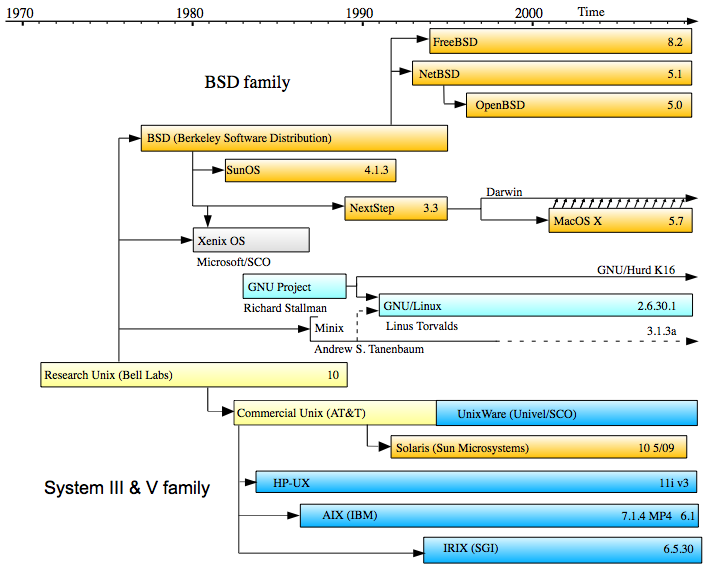
\includegraphics[width=0.75\textwidth]{02/pics/unix_history}
	\caption[Unix genealogy tree]{A partial Unix genealogy tree.
		\label{fig:unix-history}}
\end{figure}

Parallel to the development of the various Unix
flavors evolved a set of standards that helped define
how exactly the operating system should behave, what
interfaces it should provide and what kinds of
assumptions third-party software could make about the
environment.  These standards became to be known as
the ``Single UNIX Specification\index{Single UNIX
Specification}'' (SUS, commonly referred by version,
such as SUSv3) and eventually as
``\glslink{posix}{POSIX}\index{POSIX}'' (for
``Portable Operating System Interface for uniX'').
The SUS was used to qualify operating systems for the
name ``\textsc{UNIX}\index{UNIX}'' -- this
certification was obtained only by a relatively small
number of systems, since it was costly and required
re-certification of the system after any significant
change (i.e., major OS release), something that Open
Source projects, such as the BSDs certainly could not
afford.

Eventually, SUSv3 and POSIX:2001 (formally known as
\glslink{ieee}{IEEE} 1003\index{IEEE 1003}.1-2001)
became more or less interchangable; we will commonly
refer to systems or interfaces as being
``POSIX-compliant'' (or not, as the case may be).  At
the time of this writing, the latest version is
POSIX:2008\cite{history:posix2008}, which is divided
into a {\em Base Definition}, the {\em System
Interfaces and Headers}, and the {\em Commands and
Utilities}.  It should be mentioned, though, that
not only is ``the nice thing about standards that you
have so many to choose
from''\cite{history:tanenbaum-standards}, as an old
phrase coined by Andrew S.
Tanenbaum\index[names]{Tanenbaum, Andrew S.} goes,
but also that a recommendation or requirement does not
necessarily have to make sense or be realistic to be
included in a standard.  We will occasionally notice
discrepancies between what POSIX demands and what
different OS vendors chose to implement.  As two
entertaining examples, please refer to the section of
the \manpage{fcntl(2)} manual page on e.g. a NetBSD
system\cite{history:fcntl} that elaborates on the
locking semantics or the fact that POSIX could be
interpreted to require a \manpage{cd(1)} {\em
executable}\footnote{If the problem of a {\tt cd(1)}
{\em executable} isn't immediately obvious to you...
well, see Problem \ref{prob:cd}!}.

\subsection{Networking}
\label{unix:networking}

No review of the history and basic features of the
Unix operating system would be complete without a
mention of the parallel evolution of the Internet.  As
we noted in Section \ref{unix:history:os}, the
development of the Unix system and that of the
predecessors of what ultimately became the Internet
were not only related, but became inseparably merged.
The ARPANET\index{ARPANET} implemented the concept of
{\em packet switching\index{packet switching}},
allowing payload to be broken into small {\em
datagrams} and routed along different paths; its
adoption of TCP/IP\cite{history:cerf-kahn:tcp} as its
protocol suite effectively marked the beginning of the
modern Internet.  Even though some companies developed
their own TCP/IP stack, the code included in the
Berkeley Software Distribution quickly became the most
widely used implemention and ultimately replaced other
network protocols\footnote{Microsoft, for example, did
not include TCP/IP in their operating systems until
Windows 95, allowing other companies to sell their
implementations as add-on software.  The move from
their native  NetBIOS\index{NetBIOS} protocol to the
BSD derived TCP/IP stack helped make the latter the
de-facto Internet standard protocol suite.}.

In the early days of the Internet, the various
different networks -- ARPANET,
\glslink{csnet}{CSNET}\index{CSNET},
\glslink{milnet}{MILNET}\index{MILNET},
\glslink{nsfnet}{NSFNET}\index{NSFNET},
\glslink{nsi}{NSI}\index{NSI}, etc. -- were connected
via specific gateway hosts, and email exchanges as
well as communications on the early
\glslink{bbs}{BBS}\index{BBS}es and
Usenet\index{Usenet} were performed via
\manpage{UUCP}, the {\em Unix-to-Unix Copy}
tools\footnote{Every now and then you may encounter
a scruffy oldtimer who insists on pointing out that
their email address is something along the lines of
``...!orgserver!deptserv!mybox!user''. You can
trivially impress them by calling it their ``bang
path'' and agreeing that @-based email addresses are
newfangled humbug.}.  Once hosts were more frequently
directly connected to the Internet,
\glslink{smtp}{SMTP}\index{SMTP} and NNTP\index{NNTP}
became more widely used, leading to Unix servers
running various so-called  d\ae mon\index{d\ae mon}s
to provide network services as part of their normal
operations.  \\

But even before the advent of the Internet, Unix
included networking capabilities.  Through its layers
of abstraction it was possible to implement support
for different networking technologies and allow
applications to be network protocol agnostic.  In
fact, some applications, such as  email\index{email}
were available and in use prior to any traditional
networking capabilities.  The nature of Unix as a
multiuser system lead to the development of tools,
amongst them the \manpage{mail(1)} program, to allow
these users to communicate efficiently with one
another and across systems.  We will frequently review
how the nature of a scalable tool allows it to
function equally well regardless of where input data
comes from or what transport mechanism is used; a
simple, well defined program can deliver mail on a
single system while relying on a separate transport
service (i.e., UUCP or SMTP) to handle connections
with other systems.

Furthermore, the software implementing such services
was developed on and then included in the Unix
operating system.  As a result, the Internet and its
infrastructure were growing in parallel to the
capabilities of Unix, one enabling the other to become
more powerful and ubiquitous. And so today, the
overwhelming majority of the systems powering the core
infrastructure components of the Internet, such as,
for example, the \glslink{dns}{DNS} root
servers\index{Domain Name System!root servers} or most
web- and mail servers, are running on a Unix
variant\footnote{As noted in the introduction, we
continue to count Linux as a ``Unix variant'' to avoid
constant repition of the phrase ``Unix or Linux''.}:
the by far most popular implementation of the DNS
specification is, not surprisingly, the {\em
\gls{bind}} server\cite{history:dns-survey};
\manpage{sendmail}, \manpage{exim}, and
\manpage{postfix} push the majority of the world's
email\cite{history:esoft-mx}; the
\manpage{apache}\index{\tt apache} web server
still handles more than 45\% of all
\glslink{http}{HTTP} traffic on active sites than any
other web server\cite{history:netcraft-http}.


\subsection{Open Source}
\label{unix:open-source}

Unix is an inherently open system.  Developed at a
renowned research institution, it was released and
licensed together with the source code long before the
formal idea of ``Open Source\index{Open Source}'' had
manifested itself.  As we have seen in Section
\ref{unix:history}, the availability of the source
code made it possible for other various commercial
versions to be developed by different companies, but
it also allowed the development of the \gls{bsd} with
its distinctly permissive licensing terms.

Having access to the source code of the operating
system and all the tools in use is a foreign concept
in the world of proprietary software, where the source
code is guarded as a trade secret, the pillar upon
which a traditional company builds its entire profit
model.  Within the academic world in which Unix was
developed, however, access to the source code was only
natural.  Peer review and openness were fundamental
parts of this world and the system was targeted
towards engineers, hackers, advanced users who would
naturally like to make changes to tools, who would
want to extend the capabilities and add new features.

This wish to share one's work with others, to allow
others to take full advantage of it, and to make their
own modifications took two distinct directions early
on, embodied in the two open source license models
that have remained dominant to this day.  On the one
hand, the distinctly academic
BSD-License\index{BSD!License} (see Listing
\ref{code:bsdlicense}) allowed for any use of the
software whatsoever (including modification and
commercial re-selling of the products) so long as
credit was given where credit was due.  On the other
hand, the \gls{gpl}\index{GPL}, written by Richard
Stallman\index[names]{Richard Stallman} intended to
very specifically not only {\em grant}, but to {\em
enforce} certain freedoms using a moral argument.
This license, somewhat ironically, imposes a number of
restrictions on what you can do with the source code
you have received, most notably the requirement to
make public under {\em the same} license any changes
you distribute.

People have argued about the benefits of one license
over the other for decades by now, and we will not
attempt to resolve the dispute in this book.  They
represent different approaches to one's software,
perhaps a personal choice of how one wishes that it be
used in the future.  Suffice it to say that there is
incredible software licensed using both approaches,
and both models thrive to this day.  A similar
discussion involves the concept of cost and freedom
with regards to software (``Free as in beer versus
free as in speech'').  Open Source software, like all
software, comes at a price: a relatively small
component of the total cost of ownership is the actual
purchase price, and access to the source code (which
in some cases may well come under specific terms of
the license with commercial and/or closed source
software) is somewhat independent thereof.  What's
more important -- within the context of this book,
anyway -- is that the very concept of Open Source is
embedded in the Unix philosophy and culture, and as a
result System Administrators frequently {\em expect}
to be able to analyze the source code to the
applications and operating systems they run.

But not only are we {\em able} to inspect how a piece
of software works, we {\em need} to.  All too
frequently do we encounter problems or try to analyze
a system's behaviour where the question of what on
earth might be going on is answered with this advice:
``Use the source, Luke!'' -- Unix has let us do
precisely that since the beginning.\footnote{It should
be mentioned that the various commercial Unix versions
represent closed source systems.  But not only are
Open Source Unix versions nowadays much more widely in
use, virtually all of the core software running {\em
on top} of the (commercial, closed, open, or any
other) OS traditionally comes with its source code.}


\section{Basic Unix Concepts and Features}
\label{unix:basics}

The Unix operating system consists, somewhat
simplified, of three major components: a {\em kernel},
which controls the hardware, schedules tasks, and
interfaces with the various devices; a set of {\em
libraries}, which provide an interface to the kernel
(in the form of {\em  system calls\index{system
calls}} that run in privileged kernel space as well as
unprivileged {\em library functions} running in user
space); and a set of {\em tools and applications}
(often referred to as the ``userland'') using these
libraries to provide functionality to the end user.

Most Unix flavors use a {\em
monolithic}\index{kernel!monolithic} kernel, but allow
for dynamically loaded kernel
modules\index{kernel!loadable modules}.\footnote{A
discussion of {\em microkernels}\index{microkernel},
{\em unikernels}\index{unikernel}, and the various
{\em containers} that became popular in more recent
years is, unfortunately, well beyond the scope of this
chapter.  The broad subject matter of System
Administration again forces us to focus on the general
principles first.}    This approach allows for a
reduction of the kernel footprint and increased
flexibility, as device driver support can be added or
removed at runtime without requiring a reboot.  The
kernel, managing the system's resources, is running in
supervisor mode and exposes facilities via system
calls.  It is desirable to keep the number of these
entry points into kernel space limited and let
higher-level library functions provide added
functionality executed in unprivileged mode.
Therefore, most Unix versions have only a
comparatively small number of system calls: as of
January 2017,  NetBSD\index{NetBSD}, for example, had
only around 482 such
calls\cite{history:nbsd-syscalls}, with only minimal
expected growth\footnote{Revisiting an earlier draft
of this chapter from January 2012 listed 472 system
calls.  That is, over the course of five years, only
ten new system calls were added.}.

Utilizing these system calls and library functions,
the higher level tools and applications are able to
interface with the kernel and execute on the user's
behalf.  These binaries then can be divided into a
number of categories, such as executables essential
for the basic operation of the system, tools primarily
intended for use by the system administrator, and
general purpose utilities.  We will revisit this
topic in more detail in Chapter
\ref{chap:software-installation}.

\subsection{The shell}
\label{unix:basics:shell}

The Unix {\em shell}, while in many ways nothing but a
regular executable, takes a special place in the list
of utilities and commands available on the system.
The shell provides the primary user interface,
allowing for the invocation and execution of the other
tools.  AT\&T's Version 7 Unix included the so-called
``Bourne shell''\index{shell!Bourne} (named after
Steven Bourne\index[names]{Bourne, Steven}) installed
as {\tt /bin/sh}.  In addition to the ability to
invoke other commands, the shell was designed as a
{\em command interpreter} both for interactive use as
well as for {\em non}-interactive use.  That is, it
included a scripting language, allowing for complex
series of commands to be executed; for example, by
system startup scripts at boot time.\footnote{It is
worth noting that the early Bourne shell also included
support for pipelines (invented by Douglas McIlroy and
added to Unix by Ken Thompson in 1973).}

\begin{lstlisting}[float,label=code:io-redir,caption=Simple I/O redirection in the shell]
$ cmd >output          # redirection of stdout to a file
$ cmd >/dev/null       # suppression of output
$ cmd >/dev/null 2>&1  # suppression of all output
$ cmd <input           # accepting input from a file
$ cmd1 | cmd2          # feeding output from cmd1 into cmd2

# Of course these redirections can be combined...
$ cmd1 2>/dev/null | cmd2 | cmd3 2>&1 | cmd4 >file 2>output
\end{lstlisting}


Various other shells have been created since then,
mostly following either the general Bourne shell
syntax or that of Bill Joy's\index[names]{Joy, Bill} C
\manpage{csh(1)} Shell.  The most notable shells
today include: the Almquist shell \manpage{ash(1)}, a
BSD-licensed replacement for the Bourne shell,
frequently installed as {\tt /bin/sh} on these
systems; the GNU Project's Bourne-again
shell\index{shell!Bourne-again} \manpage{bash(1)},
which is the default shell on most Linux systems and
known for a large number of added features; the Korn
shell \manpage{ksh(1)}, named after David
Korn\index[names]{Korn, David} and which became the
basis for the POSIX shell standard; the TENEX C
shell \manpage{tcsh(1)}, a C shell variant developed
at Carnegie Mellon University\index{Carnegie Mellon
University}; and perhaps the Z shell \manpage{zsh(1)}
another very feature rich Bourne shell variant.

As a scripting language and due to its availability on
virtually every Unix flavor, {\tt /bin/sh} is assumed
to be the lowest common denominator: a Bourne- or
Bourne-compatible shell.  On Linux, {\tt bash(1)} is
typically installed as both {\tt /bin/bash} and {\tt
/bin/sh}, and it behaves (somewhat) accordingly based
on how it was invoked.  Unfortunately, though, its
ubiquity on Linux systems has led to a shell scripts
masquerading as {\tt /bin/sh} compatible scripts that
are, in fact, making use of {\tt bash(1)} extensions
or rely on {\tt bash(1)} compatibility and syntax.
This becomes frustrating to debug when trying to run
such scripts on a platform with a POSIX compliant {\tt
/bin/sh}.  \\

All Unix shells include the ability to perform  I/O
redirection\index{I/O redirection}.  Each program has
a set of input and output channels that allow it to
communicate with other programs.  Like the concept of
the pipe, these streams have been part of Unix's
design from early on and contribute significantly to
the consistent user interface provided by all standard
tools:  a program accepts input from {\em standard
input} (or \manpage{stdin}) and generates output on
{\em standard output} (or \manpage{stdout}); error
messages are printed to a separate stream, {\em
standard error} (or \manpage{stderr}).

The shell allows the user to change what these streams
are connected to; the most trivial redirections are
the collection of output in a file, the suppression of
output, acceptance of input from a file, and of course
the connection of one program's output stream to
another program's input stream via a pipe (see
Listing \ref{code:io-redir} for Bourne-shell
compatible examples).

The concept of these simple data streams being
provided by the operating system was inherent in the
Unix philosophy\index{Unix!Philosophy}: it provided
abstraction of interfaces, reduced overall complexity
of all tools using these interfaces, and dictated a
simple text stream as the preferred means of
communication.  We will have more to say on the Unix
philosophy in Section \ref{unix:philosophy}.

\begin{figure}[t]
	\centering
	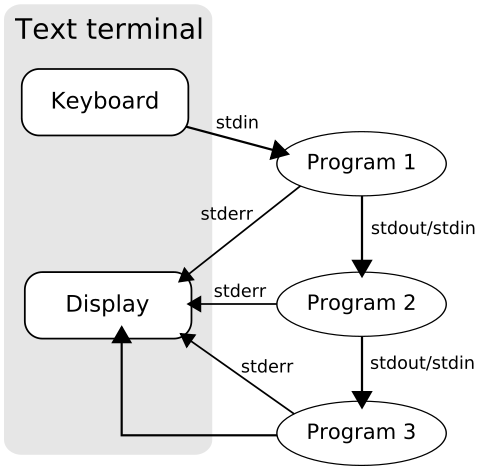
\includegraphics[width=0.5\textwidth]{02/pics/pipeline}
	\caption{Standard streams in a simple pipeline
		\label{fig:streams-pipeline}}
\end{figure}


Finally, the unix shell provides for {\em  job
control}\index{job control}, a necessity for a
multitasking operating system.  When a user logs into
the system, their {\em  login shell}\index{login
shell} is started, serving as the primary interface
between the user and the OS.  After entering a command
or a pipeline, the shell will create (``fork'') a new
process and then execute the given programs.  The
standard streams are connected as illustrated in
Figure \ref{fig:streams-pipeline}.  While the program
or pipeline is running, the user cannot do anything
else -- she has to wait until the command completes
and control is returned to the shell.  In the mean
time, all she can do is twiddle her thumbs; so much
for multitasking!

\begin{lstlisting}[float,label=code:sh-jobcontrol,caption=Simple job control in the shell]
$ cmd1 &            # send cmd1 to the background
[1] 5836            # report job number and process ID
$ cmd2 | cmd3 &     # send a process group to the background
[2] 5912
$ jobs              # report on running jobs
[1]  Running    cmd1
[2]  Running    cmd2 | cmd3
$ fg %1             # bring job 1 to the foreground
cmd1
^Z                  # suspend via Control+Z
[1]+ Stopped    cmd1
$ bg                # send it back to the background
[1]+ cmd1
$                   # hit return again...
[1]+ Done       cmd1
$                   # cmd1 has completed
\end{lstlisting}

To avoid this scenario, the C shell implemented a
feature that was quickly incorporated in the Bourne
shell, which allows users to start and control
multiple concurrent processes by placing them into the
{\em background} (by adding the {\tt \&} symbol at the
end of the command or via the shell {\tt builtin}s),
bringing them to the {\em foreground} (via {\tt
builtin}s), suspending and continuing them (by sending
possibly keyboard generated signals to the relevant
process group), etc.  Listing \ref{code:sh-jobcontrol}
illustrates the basic job control functionality.

\subsection{Manual pages and documentation}
\label{unix:basics:manual}

Another important feature of the Unix operating system
was that it included what came to be known as the
``online manual pages''\index{Manual
Pages}\footnote{In Unix's historic context,
``online'' initially meant that the documentation is
available on the running system, not ``on the
Internet''.}, reference documentation readily
available on the running system and that went beyond
just attesting to the existence of a command or
feature, but instead provided actually useful
information, including the correct invocation,
possible options, a description of the tool's
functionality as well as any known bugs.  Divided into
several sections by topic,  system calls are
documented in section two, library functions in
section three, while commands and executables are
usually documented in section one for general purpose
tools and section eight (on BSD, section {\tt 1M} on
SysV derived systems) for system administration
related commands and d\ae mons.

The standard for this documentation has always been
high, reflecting the academic culture behind the
operating system.  Rather than treat the user as a
naive consumer, Unix documentation acknowledges the
fact that the target audience consists of skilled
engineers who appreciate and require an accurate
description of the tools at their disposal in order to
make the most of them.  It may not surprise you to
know that the adoption of Unix within the Bell
Labs\index{Bell Laboratories} patent office, which
secured funding for further development, was largely
thanks to the system's abilities to typeset beautiful
documents using the {\em roff} text formatting
program\footnote{Consider that W. Richard
Stevens\index[names]{Stevens, W.  Richard} used to
typeset his famous books ``Advanced Programming in the
UNIX Environment'' and the ``TCP/IP Illustrated''
series by himself using {\tt groff(1)}.}.  The same
tools are still used to format the manual pages.

Unix provided manual pages and documentation not just
of the executables and configuration files provided by
the system, but also for so-called ``supplementary''
documents.  These comprise a number of papers that,
as in the case of the \gls{ipc}\index{IPC} tutorials,
for example, served as the de-facto reference
documentation and continue to be used in countless
Computer Science classes today to teach students the
fundamentals of Unix IPC.  Other highlights include an
introduction to the GNU debugger {\tt gdb}, the {\tt
make} tool, a \manpage{vi(1)} reference manual, an
overview of the file system, and various d\ae mons.
Since these documents are licensed under the
permissive  BSD License\index{BSD!License}, they can
be -- and thankfully are! -- included in modern Unix
versions (such as e.g. NetBSD\index{NetBSD}) and made
available on the Internet\cite{history:nbsd-docs}.

\begin{sidenote}
{\bf Understanding the Shell} \\
A System Administrator spends a significant amount of
time in the shell, both her own login shell as well as
various others.  Not only does she need to run
countless commands to remotely administrate various
hosts, she also routinely writes small, large,
complex, simple, elegant or convoluted scripts to
accomplish any thinkable task.  It is therefore
imperative to understand how the Unix shell works on a
detailed level.  It is surprising how frequently the
many intricacies of I/O redirection, of job control
and pipelines, of aliases and {\tt builtin}s taking
precedence over commands, as well as other seemingly
obscure problems manifest themselves. \\ [10pt]

If you have a background in C programming, consider
writing a general purpose Unix shell from scratch --
it will teach you invaluable lessons about how the
system works on a very fundamental level.  (If you do
not have a background in C programming... develop
one!)
\end{sidenote}



\subsection{A portable, multitasking, multiuser system}
\label{unix:basics:multi}

The Unix operating system was, from the very
beginning, designed as a {\em portable}, {\em
multitasking}, {\em multiuser} system.  These inherent
features are largely responsible for the incredible
success of this over 40 year old system and each has
wide-reaching consequences.  Initially developed on a
PDP-7\index{PDP-7} and then a PDP-11\index{PDP-11}
machine, Unix was rewritten in the C\index{C}
programming language, which allowed it to be ported
with comparatively little effort to various other
machines and hardware architectures. Figure
\ref{fig:portability} shows a few different hardware
platforms, each running a version of Unix.  Prior to
this, operating systems were written in assembly, and
that was that -- only a fool would attempt otherwise!
But as a result of this bold move to stray from
convention and instead to apply a fundamental design
choice of abstraction of complexity, the system became
inherently portable: software {\em for} Unix -- any
Unix, really -- can usually be adapted to other Unix
flavors with few modifications.

\begin{figure}[t]
	\centering
	\begin{minipage}{.4\linewidth}
		\centering
		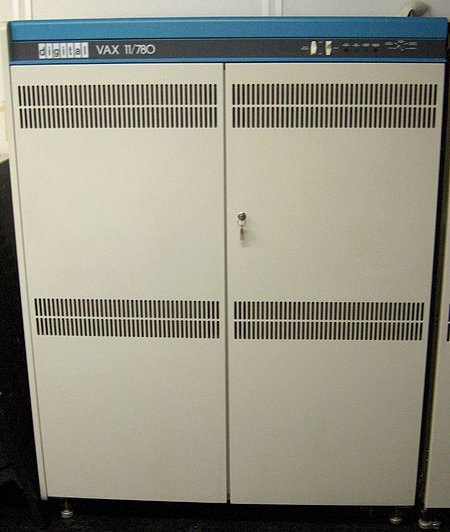
\includegraphics[width=0.9\textwidth]{02/pics/VAX_11-780_intero}
	\end{minipage}
	\hfill
	\begin{minipage}{.4\linewidth}
		\centering
		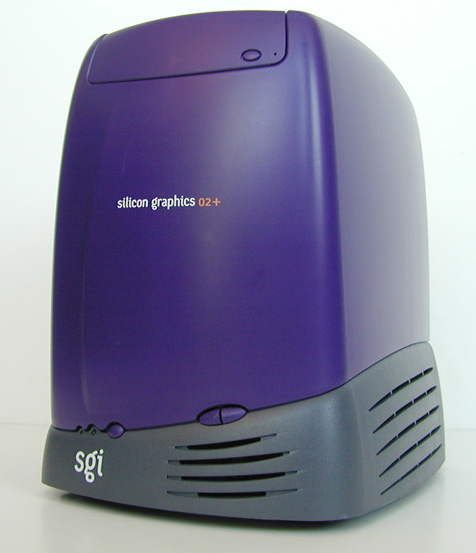
\includegraphics[width=0.9\textwidth]{02/pics/Silicon_Graphics_O2_Plus}
	\end{minipage}
	\\
	\begin{minipage}{.4\linewidth}
		\centering
		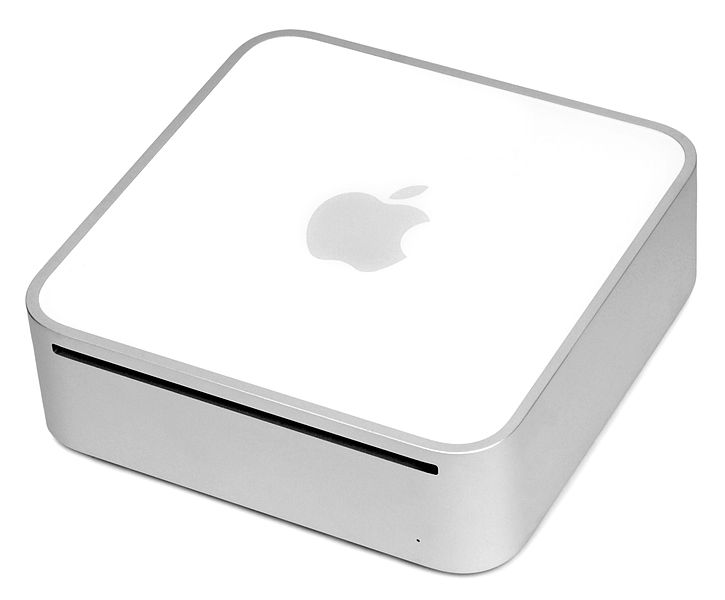
\includegraphics[width=0.9\textwidth]{02/pics/Mac-mini-1st-gen}
	\end{minipage}
	\hfill
	\begin{minipage}{.4\linewidth}
		\centering
		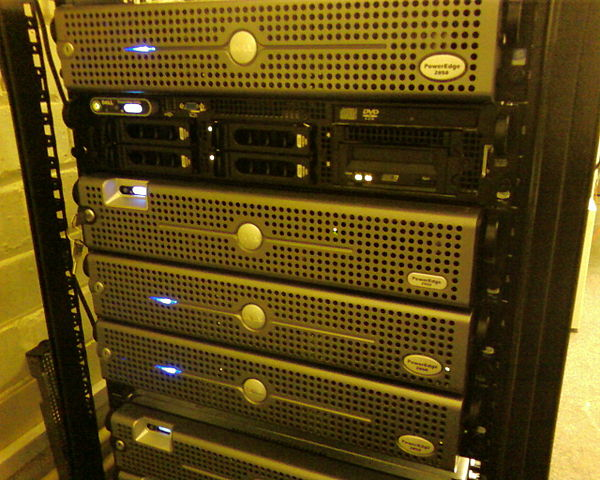
\includegraphics[width=0.9\textwidth]{02/pics/Dellpoweredge2950}
	\end{minipage}
	\caption[Different systems running Unix]{
			Different systems and architectures running Unix.
			A VAX-11 by DEC (VAX), an O2 by SGI (MIPS),
			a Mac Mini by Apple (PowerPC), PowerEdge
			servers by Dell (x86).
				\label{fig:portability}}
\end{figure}


Now, to state that Unix is {\em portable} does not
mean that one can trivially recompile the software
without any changes -- far from it!  Any System
Administrator can relate stories of having spent
hours wrangling Makefile\index{Makefile}s, {\tt
autoconf}/{\tt automake}\index{\tt autoconf}\index{\tt
automake} frameworks, and hunting down header files
and libraries.  But in the end, it remains
relatively easy to get the software to work, since all
Unix systems follow (to some degree, anyway) certain
standards and conventions.  Consider the effort of
adapting a complex piece of software from running on
Linux to, say, IRIX\index{IRIX} to that from running
on Windows 95 to Mac OS 9!  Unix having been rewritten
in the higher level C programming language, the
standardization of C, as well as the POSIX guidelines
really allowed a world of portable, flexible software
to flourish.

The {\em multitasking} nature of the Unix operating
system was a given, as it was intended to be a
time-sharing system, allowing multiple processes to
use the given resources seemingly simultaneously by
means of a scheduler which initiates context switches
to grant each process time on the
\gls{cpu}\index{CPU}.  Allowing for multiple
(simultaneous) users was just a logical consequence.
Nowadays it may not seem worth mentioning, but it is
worth noting that this system, conceived to allow
multiple users simultaneous access was designed over
40 years ago.  In comparison, Windows NT\index{Windows
NT}, first released in 1993, was the first of
Microsoft's family of operating systems to eventually
introduce multiuser capabilities, around 20 years
later; Apple\index{Apple}'s Mac OS gained multiuser
capabilities only with OS X\index{OS X} in 2001.

The nature of a {\em multiuser} system has a number of
significant implications:  A system that allows
multiple users to simultaneously utilize the given
resources is in need of a security model that allows
for a distinction of access levels or privileges.  The
system needs to be able to distinguish between file
access or resource utilization amongst users, thus
requiring the concept of access permissions, process
and file ownership, process priorities and the like.
Controlling access to shared resources by individual
users also required, effectively, a single omnipotent
user to control and administer these privileges, thus
necessitating the superuser or {\tt root
account\index{root account}} (with plenty of security
implications and concerns of its own).

In order to meet these requirements, the Unix system
uses a set of file permissions to restrict three
different types of access -- read, write and execute
(or {\tt rwx}, respectively) -- to the file {\em
owner} or {\em user}, members of a specific user {\em
group}, or everybody else (i.e., {\em others}) on the
system ({\tt ugo}, respectively).  These permissions
can be used to implement efficiently various security
models, but at the same time they are simple and
flexible enough to allow users to make their own
choices.\footnote{Different Unix versions have since
developed support for extended file
attributes\index{File Systems!Extended attributes}
including e.g. a per-file \gls{acl}\index{Access
Control Lists}, allowing the user
to wield more fine-grained control.  This is
implemented on different operating systems and in
different file systems, and the details and semantics
differ. In the interest of simplification and focusing
on the fundamental principles, we are not covering
\gls{acl}s.}

Unix has a long tradition of following the {\em
principle of least privilege}\index{Security!Principle
of Least Authority}: system services are usually run
using a dedicated user account, allowing the System
Administrator to separate file access and resource
usage such that even if the service was compromised,
harm would be minimized.  This practice translates
to routine tasks in system administration and standard
operating procedures alike.  We will revisit this
concept in more detail in Chapter \ref{chap:security}.

Processes, like files, are associated with individual
users, though privilege escalation\index{privilege
escalation} can be accomplished by means of changing
the {\em effective user ID}\index{EUID}\index{\tt
setuid(2)}.  Processes also may have specific resource
limitations, which the superuser can set system-wide
or on a per-user or per-group basis.  We will revisit
the associated system calls and commands like
\manpage{getrlimit(2)}, \manpage{sysctl(8)},
\manpage{ulimit(1)}, and {\em login
classes}\index{login classes} (see
\manpage{login.conf(5)}, where available) in Chapter
\ref{chap:monitoring} and elsewhere.

\subsection{The Unix Philosophy}
\label{unix:philosophy}

The design of the Unix operating system was based on
principles that not only have been proven time and
again to lead to stable, scalable and robust
solutions, but that have formed the basis of a
specific Unix culture\index{Unix!culture}, a way of doing things that
speaks to advanced users such as System Administrators
in particular.  You can find a thorough explanation of
this culture in classic texts such as
Kernighan\index[names]{Kernighan, Brian W.} and
Pike's\index[names]{Pike, Rob} ``The UNIX Programming
Environment''\cite{history:kernighan-pike-upe}, Eric
S.  Raymond's\index[names]{Raymond, Eric S.} ``The Art of Unix
Programming''\cite{history:esr-taoup}, or simply by
searching the Internet for the term ``Unix
philosophy'', but it warrants summarizing due to the
profound impact it has.

At its core, the  Unix
philosophy\index{Unix!Philosophy} stipulates that
tools should be kept simple and adhere to specific
simple guidelines and implement an equally simple
interface (namely text streams).  Virtually every one
of the great minds involved in the initial invention
and continued development of the Unix operating
system -- from Douglas McIlroy\index[names]{McIlroy,
Douglas} to Rob Pike\index[names]{Pike, Rob}, from
Dennis Ritchie to Ken Thompson -- can be quoted to
underline this point; they must have been on to
something.

The most well-known expression of what makes Unix Unix
is probably Douglas McIlroy's\index[names]{McIlroy,
Douglas}
summary\cite{history:mcilroy-unix-philosophy},
partially cited in the previous chapter:

\begin{quote}
{\em Write programs that do one thing and do it well. Write programs to work
together. Write programs to handle text streams, because that is a
universal interface.}
\end{quote}

This is frequently succinctly described as the KISS
(``Keep it simple, stupid'') principle and correlated
with Richard P. Gabriel's\index[names]{Gabriel,
Richard P.} ``Worse is Better\index{Worse is
Better}''\cite{history:gabriel-worse-is-better} design
philosophy, according to which simplicity is to be
preferred over all other attributes of software, at
times even including correctness.  While I do not tire
of repeating precisely this advice, I believe that the
existing literature tends to overlook, one major
factor that helped arrive at the mantra of simplicity:
deference to the user.

One of the smartest insights a program or system
developer can have is that even though they are the
person writing the software, they cannot foresee all
possible uses of the software.  They cannot know what
the user will want to accomplish or in what ways she
may wish to use the tool.  And therein lies the crux:
if I wish to enable the user to utilize the tool in
any way they wish, how can I possibly keep it simple?
Wouldn't it have to end up being a general purpose
tool, with countless inherent complexities as I
attempt to anticipate every interface of the future?
Remember, a ``general purpose product is harder to
design well than a special-purpose
one.''\cite{history:brooks-design}

This is where the Unix philosophy comes in: by
imposing restrictions, it counterintuitively opens up
the most flexible, the widest use.  Simple tools that
perform a single task and operate on a well-defined
interface are less complex than software that attempts
to keep state in deeply nested data structures (or,
worse yet: binary objects stored in files).  Our users
gain the ability to use the tools for purposes we did
not initially anticipate.  Unix grants the user
flexibility.  For  better or worse, Unix trusts its
users to know what they're doing and will happily let
you shoot yourself in the foot.

\begin{quote}
{\em \textsc{UNIX}\index{UNIX} was not designed to
stop its users from doing stupid things, as that would
also stop them from doing clever things.} -- Doug
Gwyn\index[names]{Gwyn, Doug}
\end{quote}



The awareness that your software might be used in ways
you cannot imagine, that the user of the software
might actually know better what they may wish to
accomplish than the designer or implementer is what
makes Unix so fascinating.  Interestingly, this
philosophy, this trust into the user and his or her
capabilities and knowledge stands in stark contrast
to that of the late Steve Jobs\index[names]{Jobs,
Steve}, who famously quipped that ``people don't know
what they want until you show it to
them''\cite{history:jobs}.  Apple's products are known
for their elegance and ease of use, but advanced users
know that should you attempt to do something with them
that the designers did not anticipate, it's either
impossible or painfully cumbersome.

The primary user interface on the Unix systems remains
the command-line\glslink{cli}.  This is not for a lack
of other options, but a manifestation of the Unix
philosophy.  While it may appear more
``user-friendly'' to a novice to use a pointing device
to select pre-determined options from a menu using a
\gls{gui}, it is anathema to efficient System
Administration.

System Administrators need to be able to perform tasks
remotely, quickly, and reliably unattended; execution
of programs needs to be automated and scheduled,
configuration be done outside of the application, and
data be transformed with the myriad of available
filters.  As you can tell, these requirements go back
to the Unix way of writing simple tools that work well
together by communicating via text streams.
Thanks to the consistency with which these principles
are implemented across the platform, the learning
curve for advanced users, while perhaps steeper than
on some other systems, only needs to be climbed
once.  At the same time, it gets you to a higher level
of efficiency quickly.  \\

The ability to combine individual tools to build
larger, more complex ones; to remotely access hundreds
or thousands of systems in the same manner as one
would a single system; to allow rapid development of
simple prototypes constructed of growing pipelines; to
be able to control access to shared resources
following a simple yet flexible security model; to
extend and tune the operating system itself; to be
able to do all the things that the designers of the
system could not have envisioned you doing -- this
power is what Unix confers upon the advanced user.  It
is why System Administrators not only prefer Unix, but
actually enjoy working on this platform.

\begin{lstlisting}[float,label=code:bsdlicense,caption={[2-clause
BSD license]The simplified, or 2-clause, BSD license.
Nice and terse, huh?  In contrast, the \gls{gnu}
\gls{gpl} clocks in at 11 full text pages.}] 
Copyright (c) <year>, <copyright holder>
All rights reserved.

Redistribution and use in source and binary forms, with or
without modification, are permitted provided that the
following conditions are met:

1. Redistributions of source code must retain the above
   copyright notice, this list of conditions and the
   following disclaimer.
2. Redistributions in binary form must reproduce the
   above copyright notice, this list of conditions and
   the following disclaimer in the documentation and/or
   other materials provided with the distribution.

THIS SOFTWARE IS PROVIDED BY THE COPYRIGHT HOLDERS AND
CONTRIBUTORS "AS IS" AND ANY EXPRESS OR IMPLIED
WARRANTIES, INCLUDING, BUT NOT LIMITED TO, THE IMPLIED
WARRANTIES OF MERCHANTABILITY AND FITNESS FOR A PARTICULAR
PURPOSE ARE DISCLAIMED. IN NO EVENT SHALL THE COPYRIGHT
OWNER OR CONTRIBUTORS BE LIABLE FOR ANY DIRECT, INDIRECT,
INCIDENTAL, SPECIAL, EXEMPLARY, OR CONSEQUENTIAL DAMAGES
(INCLUDING, BUT NOT LIMITED TO, PROCUREMENT OF SUBSTITUTE
GOODS OR SERVICES; LOSS OF USE, DATA, OR PROFITS; OR
BUSINESS INTERRUPTION) HOWEVER CAUSED AND ON ANY THEORY
OF LIABILITY, WHETHER IN CONTRACT, STRICT LIABILITY, OR
TORT (INCLUDING NEGLIGENCE OR OTHERWISE) ARISING IN ANY
WAY OUT OF THE USE OF THIS SOFTWARE, EVEN IF ADVISED OF
THE POSSIBILITY OF SUCH DAMAGE.

The views and conclusions contained in the software and
documentation are those of the authors and should not be
interpreted as representing official policies, either
expressed or implied, of <the project>.
\end{lstlisting}

\pagebreak

\chapter*{Problems and Exercises}
\addcontentsline{toc}{chapter}{Problems and Exercises}
\section*{Problems}

\begin{enumerate}
\item
Research the history of the Unix operating system in more detail.  Branch
out into the ``USL vs. BSDi'' lawsuit.  Follow the BSD genealogy into the
Mac OS X system.  Analyze the future direction of the commercial Unix
versions.

\item
Review the Linux, NetBSD and Solaris versioning numbers.  Try to correlate
specific features to specific releases across these systems (note the
different Linux distributions numbers as well).

\item
Review the {\tt intro(1)} manual pages on your system (they may exist for
different sections and, depending on the Unix flavor, in varying detail).
From there, move on to the following manual pages, considering the
multiuser implications: {\tt chmod(1)}/{\tt chown(1)}, {\tt login(1)},
{\tt passwd(5)}, {\tt su(1)}, {\tt sudo(8)}

\item
\label{prob:cd}
Does the POSIX standard really require a {\tt cd(1)} {\em executable}?  If
it did, what might be a problem with that?  Consider the environment of a
process and how a shell executes commands.

\item
Play around in the Unix environment of your choice.  Look at the
executables found in the system's path ({\tt /bin}, {\tt /usr/bin}, {\tt
/sbin}, {\tt /usr/sbin}) -- do you know what all these tools do?

\item
Review your understanding of the Unix philosophy of simple tools acting as
filters.  Does this reflect your usage of the tools you most frequently
execute?  Which tools do {\em not} work (well) as a filter?  Why?

\item
Research the design decisions underlying other popular operating systems.
In how far do they differ from those presented here?  Do they influence or
reflect the primary user base (i.e., what is cause and what is effect)?  How
do they affect or relate to System Administration, especially on a large
scale?

\end{enumerate}

\section*{Exercises}
\addcontentsline{toc}{section}{Exercises}

\begin{enumerate}
\item
Using the programming language of your choice, write a simple interactive
shell capable of executing programs on the user's behalf.  Try to use it
as your shell.  Were you aware of the limitations before you did this?
Were you aware of the complexity of even basic features?

\begin{enumerate}

\item
Compare your shell to some of the existing implementations.  What features
are missing from your shell?  How difficult do you think would it be to
implement them?

\item
Add additional features to your shell, such as support for input/output
redirection, pipelines, expansion of environment variables or job control.
(Note: this is a {\em significant} project, but you will learn a great
deal about the Unix operating system in the process.)

\item
Research and review the concept of a {\em restricted shell}.  Would
writing such a shell be {\em more} or {\em less} effort to do?
\end{enumerate}

\end{enumerate}

\pagebreak

\bibliographystyle{plainnat}
\begin{thebibliography}{99}

\bibitem{history:top500} TOP500; on the Internet at
\url{https://www.top500.org/statistics/list/}
(visited January 16, 2017)

\bibitem{history:bell-labs-unix-history}{\em The Creation of the UNIX Operating
System}, on the Internet at
\url{http://www.bell-labs.com/history/unix/}
(visited January 7, 2012)

\bibitem{history:dmr-history}Dennis M. Ritchie, 'The Evolution of the Unix
Time-sharing System', published in {\em AT\&T Bell Laboratories Technical
Journal}, ``Computing Science and Systems: The UNIX System,'' 63 No. 6
Part 2, October 1984;  also available via the Internet Archive at e.g.
\url{https://web.archive.org/web/20150408054606/http://cm.bell-labs.com/cm/cs/who/dmr/hist.html} (visited January 17, 2017)

\bibitem{history:kernighan-pike-upe}Brian W. Kernighan, Rob Pike, {\em The UNIX
Programming Environment}, Prentice Hall, 1984

\bibitem{history:esr-taoup}Eric Steven Raymond, {\em The Art of Unix Programming},
Addison-Wesley Professional, September 2003; also available on the
Internet at
\url{http://catb.org/~esr/writings/taoup/} (visited January 7, 2012)

\bibitem{history:tuhsml}The Unix Heritage Society Mailing List,
\url{http://minnie.tuhs.org/mailman/listinfo/tuhs}

\bibitem{history:adams-h2g2}Douglas Adams, {\em The Hitchhiker's Guide to the Galaxy},
Pan Books, 1979

\bibitem{history:kr}Brian W. Kernighan, Dennis M. Ritchie, {\em The C Programming
Language}, Prentice Hall, 1988

\bibitem{history:dmr-pipes}Dennis M. Ritchie, 'Advice
from Doug Mcilroy'; now only found on the Internet
Archive at
\url{https://web.archive.org/web/20150205024833/http://cm.bell-labs.com/cm/cs/who/dmr/mdmpipe.html}

\bibitem{history:mcilroy-reader}Douglas McIlroy, {\em
A Research UNIX Reader: Annotated Excerpts from the
Programmer's Manual, 1971-1986}; on the Internet at
\url{http://www.cs.dartmouth.edu/~doug/reader.pdf}

\bibitem{history:bsdisuit}'USL vs. BSDI documents', only available on the Internet Archive via e.g.
\url{https://web.archive.org/web/20150205025251/http://cm.bell-labs.com/cm/cs/who/dmr/bsdi/bsdisuit.html} (visited January
18, 2017)

\bibitem{history:torvalds-announce}'What would you like to see most in minix?',
Linus Torvalds, posting to the \url{comp.os.minix} newsgroup on Usenet, on
the Internet at
\url{https://groups.google.com/group/comp.os.minix/msg/b813d52cbc5a044b}
(visited January 16, 2012)

\bibitem{history:bsd-license}{\em BSD Licenses} on
Wikipedia at
\url{https://en.wikipedia.org/wiki/BSD\_licenses} (visited
January 18, 2017)

\bibitem{history:levenez-history}\'{E}ric L\'{e}v\'{e}nez, {\em Unix History}, on
the Internet at
\url{http://www.levenez.com/unix/} (visited January 5,
2012)

\bibitem{history:posix2008}The IEEE and The Open Group, ``The Open Group Base
Specifications Issue 7, IEEE Std 1003.1, 2016 Edition'' on the Internet at
\url{http://pubs.opengroup.org/onlinepubs/9699919799/} (visited January 17,
2017)

\bibitem{history:tanenbaum-standards}Andrew S. Tanenbaum, in 'Computer Networks',
Prentice Hall, 2004

\bibitem{history:fcntl}\manpage{fcntl(2)}, NetBSD
System Calls Manual, on the Internet at
\url{http://netbsd.gw.com/cgi-bin/man-cgi?fcntl++NetBSD-current}
(visited January 18, 2017)

\bibitem{history:nbsd-syscalls}NetBSD system call name/number ``master'' file, on
the Internet at
\url{http://cvsweb.netbsd.org/bsdweb.cgi/src/sys/kern/syscalls.master?rev=HEAD}
(visited January 18, 2017)

\bibitem{history:nbsd-docs}4.4 Berkeley Software Distribution Documentation, on
the Internet at
\url{http://www.netbsd.org/docs/bsd/lite2/} (visited
January 28, 2012)

\bibitem{history:cerf-kahn:tcp}Vinton G. Cerf, Robert E. Kahn, ``A Protocol for
Packet Network Intercommunication'', IEEE Transactions on Communications 22 (5);
also available on the Internet at
\url{http://ece.ut.ac.ir/Classpages/F84/PrincipleofNetworkDesign/Papers/CK74.pdf}
(visited January 28, 2012)

\bibitem{history:dns-survey}DNS server survey, 2004; on the Internet at
\url{http://mydns.bboy.net/survey/} (visited February 4, 2012)

\bibitem{history:esoft-mx}Mail (MX) Server Survey, August 1st, 2007, showed over
60\% of SMTP traffic to originate from a Sendmail, Exim, or Postfix
installation; on the Internet at
\url{http://www.securityspace.com/s\_survey/data/man.200707/mxsurvey.html}
(visited February 4, 2012)

\bibitem{history:netcraft-http}January 2017 Web Server Survey, on the Internet at
\url{https://news.netcraft.com/archives/2017/01/12/january-2017-web-server-survey.html}
(visited January 18, 2017)

\bibitem{history:mcilroy-unix-philosophy}M. D. McIlroy, E. N. Pinson, and B. A.
Tague {\em Unix Time-Sharing System Forward}, The Bell System Technical
Journal. Bell Laboratories, 1978

\bibitem{history:gabriel-worse-is-better}Richard P. Gabriel, ``Worse is Better'',
on the Internet at
\url{http://dreamsongs.com/RiseOfWorseIsBetter.html.html} (visited February 5,
2012)

\bibitem{history:brooks-design}Frederick P. Brooks, Jr., {\em The Design of
Design}, Addison-Wesley Professional, 2010

\bibitem{history:jobs}Steven P. Jobs, as quoted in BusinessWeek (25 May 1998)

\bibitem{history:salus-history}Peter H. Salus, {\em A Quarter Century of UNIX},
Addison-Wesley Professional, 1994

\bibitem{history:tuhs}The Unix Heritage Society, {\em The Unix Archive},
on the Internet at
\url{http://www.tuhs.org/Archive/README} (visited April 11, 2012)

\end{thebibliography}
